
\section{Chapter 1:\\ Estimating process-explicit model parameters from species distribution data using the evolutionary algorithm CMA-ES}

\vspace*{1cm}
\sffamily
\large
\begin{center}
Victor Van der Meersch$^1$, Isabelle Chuine$^1$

\vspace*{0.1cm}
\small
\emph{$^1$CEFE, Univ Montpellier, CNRS, EPHE, IRD, Montpellier, France}
\end{center}

\vspace*{0.7cm}
\normalsize
\textbf{Published in \emph{Methods in Ecology and Evolution}:\\} \url{https://doi.org/10.1111/2041-210X.14119}

\vspace*{1cm}

\textbf{ABSTRACT}\\
Two main types of species distribution models are used to project
species range shifts in future climatic conditions: correlative and
process-explicit models. Although there is some continuity between these
two types of models, they are fundamentally different in their
hypotheses (statistical relationships \emph{vs} mechanistic
relationships) and their calibration methods (correlative models tend to be
occurrence data-driven while process-explicit models tend to be prior-driven).

One of the limitations to the use of process-explicit models is the
difficulty to parameterize them for a large number of species compared
to correlative SDMs. We investigated the feasibility of using an
evolutionary algorithm (called covariance matrix adaptation evolution
strategy, CMA-ES) to calibrate process-explicit models using species
distribution data. This method is well established in some fields
(robotics, aerospace research, \ldots), but has never been used, to
our knowledge, in ecology, despite its ability to deal with very large
space dimensions. Using tree species occurrence data across Europe, we
adapted the CMA-ES algorithm to find appropriate values of model
parameters. We estimated simultaneously 27 to 77 parameters of two
process-explicit models simulating forest tree's ecophysiology for three
species with varying range sizes and geographical distributions.

CMA-ES provided parameter estimates leading to better prediction of
species distribution than parameter estimates based on experts
knowledge. Our results also revealed that some model parameters and
processes were strongly dependent, and different parameter
combinations could therefore lead to high model accuracy.

We conclude that CMA-ES is an efficient state-of-the-art method to
calibrate process-explicit models with a large number of parameters using
species occurrence data. Inverse modelling using CMA-ES is a powerful
method to calibrate process-explicit parameters which can hardly be
measured. However, the method does not warranty that parameter
estimates are correct because of several sources of bias, similarly to
correlative models, and expert knowledge is required to validate
results.

\rmfamily

\newpage

\subsection{Introduction}\label{introduction}

The speed and magnitude of projected climate changes are profoundly
affecting species distributions, ecological communities and ecosystem
processes, and numerous ecological systems are now approaching tipping
points (\citealp{Lenton2008, Barnosky2012, Steffen2018}; but see
\citealp{Brook2013}). Large
uncertainties on the persistence and the resilience of ecosystems exist.
Ecological forecasting has now become a critical tool for managers and
decision-makers \citep{Urban2015}, and
robust predictive approaches are necessary to provide reliable
projections of species geographic range shifts and ecosystem functioning
\citep{Mouquet2015}.
Forecasting the dynamics of ecological systems for the upcoming decades
and centuries is very difficult, because ecological systems are
extremely complex, influenced by a lot of factors and processes, and
climatic conditions with no analogues in the recent past are forecasted
to become common \citep{Williams2007, Radeloff2015, Fitzpatrick2018}. Ecological models have thus increased in complexity over the
last 50 years, incorporating more and more processes described with
various degrees of complexity depending on their objectives.

Nowadays, two main types of species distribution models (SDM) are used
to project species range shifts in future climatic conditions:
correlative and process-explicit models \citep{Dormann2012}. The vast majority of currently used SDMs are correlative: they seek to find
statistical relationships between various environmental descriptors and
species presence and absence. They assume there is an equilibrium
between species distribution and environment \citep[equilibrium postulate,][]{Guisan2005}, that there is no adaptive responses within a generation \citep[no trait plasticity,][]{Berzaghi2020}, and
that species niche is stable over macroevolutionary time \citep[niche conservatism,][]{Pearman2008a}. Most of them include a fairly large number of predictors
(particularly in machine-learning approaches), and consider flexible
transformations (linear, quadratic\ldots) and interactions between them
\citep{Merow2014}. Even
though some authors advocate for "\emph{putting more biology into SDMs}"
\citep{Higgins2012},
parameters have no a priori defined ecological meaning
\citep{Dormann2012} and
shape of response curves to environmental variables is generally not
constrained based on biological considerations. Although these models
are not always used correctly \citep{Araujo2019, Santini2021}, their flexibility makes them an important tool in
predictive ecology \citep{Mouquet2015}. They have been widely used especially to generate species
range projections under current and future climates \citep[e.g.][]{Guisan2005}.
Nevertheless, their ability to accurately describe the effects of
climate on species distributions has recently been questioned \citep[e.g.][]{Fourcade2018, Journe2020, Warren2021}.\\
For all these reasons, another kind of models has been developed.
Process-explicit (or process-based) models aim to translate into mathematical equations our
knowledge about the physiological and ecological processes involved in
an organism's life, such as growth, reproduction, survival, movement,
and interactions with other livebeings. Process-explicit models take more
time to develop and are more challenging to use, but they might provide
a greater comprehension of the complexity of ecosystem dynamics and more
robust projections in novel conditions
\citep{Evans2012, Zurell2016, Singer2016, Urban2016}. A wide
variety of process-explicit models exists, from quite simple models \citep[e.g.][]{Kleidon2000} to much
more complex ones \citep[e.g.][]{Dufrene2005}. They all rely on an explicit representation of
processes at stake, with a direct biological interpretation - at least
in principle \citep{Connolly2017}. Process-explicit models may also include some phenomenological
relationships on lower-level processes, but never on the pattern itself.
The choices about the specific processes to include into the model are
made based on theory, empirical observations and the objectives of the
research, and modeler subjectivity may play an important role. One of
the challenges is to build a model with the appropriate amount of
complexity: a too simplistic model might be unrealistic whereas a very
complex model could be far beyond our ability to understand it (because
of interconnected mechanisms) and calibrate it. Each model relies on
different hypotheses with its own balance of complexity, accuracy and
parsimony - and thus different numbers of unknown parameters to
calibrate. Parameter values of this kind of models are obtained with
different methods. Some of these parameters can be individually
estimated with field observations or experimental data, or are already
available in the literature. When this is not possible, groups of
parameters defining a relationship between a process variable and
environmental variables or other processes are estimated jointly using
inverse modelling methods and data on the processes modelled \citep[e.g.][]{Cailleret2020, Asse2020}.

Calibration (i.e.~parameter setting and estimation) is a fundamental
step in the modelling process. It allows the model to reproduce the
reality with more or less success. The result of the calibration
provides insights on the ability of the model to reproduce and explain
reality (model predictive power). Calibration of complex models such as
process-explicit SDMs is time-consuming, and modelers are often challenged
by the dimension of the parameter space, the complexity of the possible
correlations among parameters, and the scarcity of observed experimental
data to calibrate them. Therefore, although the philosophy of such
models is to measure parameters, statistical inference might be useful
when data are not yet available to infer parameter values. Parameter
inference can be achieved through several methods which have been
developed in the last decades. Most of them fall into two categories:
informal and statistical calibration. On the one hand, statistical
calibration assumes a data-generating model, and a likelihood function,
which quantifies the probability of the observed data given the model
parameters, is expressed mathematically. This likelihood is the
foundation of \emph{maximum likelihood estimation} and
\emph{Bayesian inference}, two commonly used methods for parameter
estimation. In practice, deriving the likelihood function can be quite
challenging for complex models with many parameters and thresholding.
One approach is to use numerical methods such as
\emph{simulation-based inference} or \emph{approximate Bayesian computation} \citep[e.g.][]{Hartig2014}. However, obtaining a reliable estimate of the
likelihood of a complex process-explicit model can require a large number
of simulated samples, which can be computationally expensive. On the
other hand, informal calibration uses an informal objective function to
measure the discrepancy between the model predictions and the observed
data. By minimizing the objective function, one is able to identify the
parameter values that best fit the observed data, even though it may not
have the same statistical rigor as statistical calibration. This
optimization step can be achieved with several methods, either
deterministic (e.g.~Nelder-Mead method) or stochastic (e.g.~simulated
annealing, evolutionary algorithms).\\
Recently, an approach belonging to the evolutionary algorithm family,
called Covariance Matrix Adaptation Evolution Strategy (CMA-ES), has
been proposed \citep{Hansen2001}. One of the advantages of CMA-ES is its ability to cumulate
information over iterations in order to adapt its own parameters (in
particular the covariance matrix), which makes it more robust to noise.
CMA-ES is especially performant for non-separable problems (i.e.~when
the model parameters are dependent) and large search space. This method
has been successfully applied in various fields such as aerospace \citep[e.g.][]{Collange2010},
optics \citep[e.g.][]{Gagne2008}, and robotics \citep[e.g.][]{Hill2020}. CMA-ES is acknowledged to be one of the most
efficient approaches in continuous black-box optimization
\citep{Hansen2010} but to
our knowledge has never been used in ecology.

Here we explored the feasibility and interests of calibrating
process-explicit SDMs with CMA-ES using species occurrence data as
correlative SDMs do \citep[fitted process-explicit models \emph{sensu}][]{Dormann2012}. We
focused on two forest process-explicit models of varying levels of
complexity to evaluate the ability of CMA-ES to calibrate such models.
The two models are PHENOFIT \citep[27 to 36 parameters,][]{Chuine2001} and
CASTANEA \citep[77 parameters,][]{Dufrene2005}. Each model also emphasizes different ecological
processes: while PHENOFIT focuses on phenology and how it relates to
survival and reproduction, CASTANEA focuses on carbon and water cycles.
We focused on three European common tree species, with different range
extent and ecological preferences in order to evaluate the algorithms
performance in various geographical and climatic conditions. European
beech (\emph{Fagus sylvatica} L.) is one of the most widely distributed
broadleaved tree in Europe (from southern Sweden to Sicily and from
Spain to northwest Turkey), holm oak (\emph{Quercus ilex} L.) is an
evergreen broadleaved tree native of the Mediterranean region, and
silver fir (\emph{Abies alba} Mill.) is a coniferous tree which mainly
occurs in mountain forests of Central Europe and some parts of Southern
and Eastern Europe.

\subsection{Material and methods}\label{methods}

\subsubsection{Process-explicit models}\label{sec:pbmodels}

All versions of the models used for this study are coded in Java and
distributed by the \href{https://capsis.cirad.fr/capsis/home}{CAPSIS}
platform.

PHENOFIT is a process-explicit species distribution model for forest tree
species which focuses on phenology. It relies on the principle that the
distribution of a tree species depends mainly on the synchronization of
its timing of development to the local climatic conditions
\citep{Chuine2001}. It is
composed of several submodels, including phenology models for leaves,
flowers and fruits, and stress resistance models. It simulates the
fitness (survival and reproductive success) of an average individual
using daily meteorological data, soil water holding capacity and species
specific parameters (see \hyperref[chap1:appendixA]{Appendix A} for
details). PHENOFIT has been validated for several North American and
European species by comparing their known distribution to the modelled
fitness \citep[e.g.][]{Morin2007, Saltre2013, Duputie2015, Gauzere2020}.

CASTANEA is an ecophysiological process-explicit model which simulates
carbon and water fluxes in forests
\citep{Dufrene2005}. The
model simulates the ecosystem as an average tree with six compartments
(leaves, branches, stem, coarse roots, fine roots and reserves). It is
much more complex than PHENOFIT, with several processes described and
computed, such as photosynthesis, stomatal opening, maintenance and
growth respiration, transpiration, and carbon allocation (see
\hyperref[chap1:appendixA]{Appendix A} for details). CASTANEA
requires daily meteorological variables and soil characteristics. The
model has been initially validated at stand scale for beech
\citep{Davi2005}, and was
then successfully applied to other European species \citep[e.g.][]{Davi2006, Delpierre2012, Davi2017}.

Both models, in their standard version (called here after expert
calibration), are parameterized using various sources of information.
Some parameters are directly measured or found in the literature such as
leaf life span, specific leaf area, LT50 (freezing temperature causing
50\% mortality) of leaves, leaf reflectance, and so on. Other parameters
cannot be measured at all, or their measurement require an enormous
effort that cannot be deployed for a large number of species. These
parameters are thus inferred by inverse modelling using either Bayesian
methods or optimizing methods and data on the specific process they are
describing. This is for example the case for phenology models for which
all parameters cannot be measured, especially those describing bud
dormancy break regulation, since no method allow to measure dormancy
break precisely so far (except for a few fruit tree species). Finally, a
few parameters are prescribed based on expert knowledge as no data to
estimate them exist. For this study, the standard versions of both
models were run for the three species using the same climatic data used
to do the inverse calibration (see \nameref{sec:climatedata}), in order to
compare the correctness of the predictions obtained with the two types
of calibration.



\hypertarget{data}{%
\subsubsection{Data for the calibration}\label{data}}

\paragraph{Climate and soil data}
\label{sec:climatedata}

Raw climatic variables were extracted from ERA5-Land hourly dataset
\citep{MunozSabater2021} from 1970 to 2000, at a
spatial resolution of 0.1 degree in latitude and longitude. We
calculated the daily mean values of the following variables used by
PHENOFIT and CASTANEA: minimum, mean and maximum daily temperatures,
mean dewpoint temperature, daily precipitation, daily global radiation
and daily mean wind speed. We computed the daily relative humidity with
the ratio of vapor pressure and saturation vapor pressure \citep[both
calculated with Clausius-Clapeyron equation) using \emph{humidity} R
package,][]{Cai2019}. Daily potential
evapotranspiration was calculated with Penman--Monteith equation (FAO
standard of hypothetical grass reference surface) using a slightly
modified version of the \emph{ET()} function in
\emph{Evapotranspiration} R package \citep{Guo2016}.

Water content at field capacity and wilting point data were extracted
from EU-SoilHydroGrids \citep{Toth2017} which is at 1km resolution. Percentage of sand, silt and
clay particles, percentage of coarse fragments, bulk density and soil
depth were extracted from SoilGrids250m
\citep{Hengl2017} at a 250m
resolution. These data (except for soil depth) are provided at seven
soil depths, so we summarized them (weighted sum or weighted mean)
taking into account each layer width and total soil depth. Finally, all
variables were upscaled at the ERA5-Land spatial resolution 0.1° using
bilinear interpolation.

\paragraph{Tree occurrence data used for the
calibration}\label{sec:occurrencedata}

Sources of occurrence data are known to differ even for common European
trees \citep{Duputie2014}
and this makes it quite challenging to gather comprehensive data at a
sufficient spatial resolution all over Europe. The occurrence data we
used essentially rely on the EU-Forest dataset
\citep{Mauri2017} which
benefits from inventory and monitoring programmes implemented in most
European countries. As EU-Forest is limited to forest ecosystems, we
combined it with presence records extracted from the Global Biodiversity
Information Facility (\citealp{GBIF2022}; see
\hyperref[chap1:appendixB]{Appendix B} for all download links) but
removing observations outside natural species ranges as defined by Atlas
Flora Europeae (AFE, \citealp{AFE2005}) and EuroVegMap \citep{EVM2003}. By doing so, we also included occurrences of
isolated native trees living outside forests, excluding records from
arboreta or gardens where the species would have been planted as an
exotic. For holm oak, we also added occurrence records in the
Mediterranean Basin from the WOODIV database
\citep{Monnet2021}, leaving
out EU-Forest and GBIF records we had already gathered. We upscaled all
species records at the ERA5-Land resolution (0.1°, see
\nameref{sec:climatedata}), i.e.~the species
is considered to be present in the cell if there is at least one record.
We finally obtained 21458 occurrence cells for beech, 6653 for holm oak
and 5385 for silver fir (see \hyperref[chap1:appendixB]{Appendix B} for details).

All the datasets described above are presence-only data. Therefore, we
generated cells where species are supposed to be absent,
i.e.~pseudo-absence cells. In order to avoid as far as possible creating
false absence data, we used EU-Forest cells where the species is not
reported present as pseudo-absence cells. We assumed that national
forest inventories were exhaustive (which is not true since only
specific forest plots in a 0.1° cell are monitored). We obtained 25423
absence cells for beech, 37931 for holm oak and 38365 for silver fir
(see \hyperref[chap1:appendixC]{Appendix C}).

We selected subsets of 2000 points (1000 presences and 1000
pseudo-absences) in order to reduce computational costs. For each
species, we generated ten presence clusters (k-means algorithm) of
similar bioclimatic conditions based on annual climate normals computed
with R package \emph{dismo} \citep{Hijmans2021} and ERA5-Land variables. In each cluster, we
randomly sampled a number of cells where the species is present
proportional to the total number of a number of cells where the species
is present in the cluster. The aim of this stratified random sampling
was to make sure that all species environmental preferences were
proportionally represented. We then randomly sampled the same number of
pseudo-absence cells (see \hyperref[chap1:appendixB]{Appendix B}).

Regarding PHENOFIT model, we calibrated ten times each species parameter
set, with 5 repetitions on 2 random subsets of
presences/pseudo-absences, except for beech. In the latter case, we ran
10 repetitions on 10 subsets (i.e.~100 calibrations) to investigate both
the effect of subsampling and the effect of stochasticity. Since
CASTANEA computing time was much higher (see \autoref{tab:modelstable}),
we ran only two calibration for each species (on 2 different random
subsets).

\clearpage

\subsubsection{Model calibration}\label{model-calibration}

\paragraph{Covariance Matrix Adaptation Evolution Strategy
principles}\label{covariance-matrix-adaptation-evolution-strategy-principles}

Covariance Matrix Adaptation Evolution Strategy (CMA-ES) is widely
accepted as a robust optimization algorithm for non-linear, non-convex,
as well as non-separated optimization problems in continuous domain
\citep{Hansen1996, Hansen2001, Hansen2006}. It is based on the
principle of evolutionary biology, via recombination, mutation and
selection of the most fit candidate solutions (i.e.~parameter sets
providing the best predictions). At each iteration:\\
- \(\lambda\) candidate solutions are evaluated, i.e.~model runs
\(\lambda\) times with \(\lambda\) different parameter sets and the
objective function is evaluated\\
- the best \(\mu\) candidate solutions are selected\\
- the weighted mean candidate solution \(m\) is computed (mean of the
best \(\mu\) parameter sets weighted by their objective function
value)\\
- covariance matrix \(C\) and step size \(\sigma\) are updated (with
information accumulated over several consecutive iterations)\\
- new \(\lambda\) candidate solutions are sampled in a normal
distribution \(\mathcal{N}(m, \sigma C)\), with both recombination (via
the favorite solution \(m\)) and mutations (via the perturbations
\(\sigma C\))\\
One of the strengths of this approach lies in the combination of
rank-\(\mu\)-update, where prior information from previous generations
is exploited (mean of the previous covariance matrices, with a higher
weight for recent generations), and cumulation, where correlations
between generations are retained in an evolution path (sum of
consecutive steps), to update the covariance matrix at each step (see
\citealp{Hansen2016} for a detailed
description of the algorithm).

\paragraph{CMA-ES in practice}\label{cma-es-in-practice}

One of the advantages of CMA-ES is that it does not require a complex
parameter tuning: as best parameter values at a given time of the
optimization process might no longer be efficient later, CMA-ES
implements an internal adaptation of its parameters. We only chose the
number of candidate solutions \(\lambda\), depending on the optimization
problem complexity (\(\mu\) was set to \(\lambda/2\)). The default
recommended value for \(\lambda\) is \(4 + 3 ln(N)\), where \(N\) is the
number of parameters to calibrate (i.e.~\(\lambda \in [14,17]\) in our
case). We set \(\lambda = 20\), in order to improve the global search
capability \citep{Hansen2004} and
take advantage of the computation power at our disposal. All model
parameters were linear scaled into \([0;10]\) so that the same standard
deviation can be applied to all parameters: here we chose \(\sigma = 2\)
(see
\href{https://cma-es.github.io/cmaes_sourcecode_page.html\#practical}{Nikolaus
Hansen personal website} for practical hints on variable encoding). Our
stopping criterion for the optimization procedure was the budget,
i.e.~the number of model runs.

For an easier use and the sake of reproducibility, we chose to use a
pure R implementation of CMA-ES available in the R package \emph{cmaes}
\citep{Trautmann2011}.
The function \emph{cma\_es()} enables us to do \(\lambda\) function
evaluations in parallel so as to substantially reduce computation time.
It also allows us to define lower and upper bound constraints, by
penalising the objective function value of the candidate solution if it
violates the boundaries. We customized the \emph{cma\_es()} function to
add an option to define death penalty constraints (rejection of the
infeasible candidate solution who is sampled again), in order to define
a range of ecologically possible solutions in terms of inequality
constraints between parameters (see
\hyperref[chap1:appendixD]{Appendix D} for details about boundaries
and constraints handling). Death penalty is the easiest way to handle
constraints when the feasible region is fairly large, but it is not
perfect as there is no use of information from infeasible points
(i.e.~points which violate the constraints).

The objective function for the calibration was the area under the
receiver operating characteristic curve (AUC), evaluated against a
subsets of 2000 points (see \nameref{sec:occurrencedata}). Although AUC has been criticized as an imperfect
measure of model performance \citep{Lobo2008, Leroy2018}, we used it as objective function because our goal here was
only to calibrate models by maximizing discriminating capacity
(i.e.~potential to correctly classify presences and absences) with a
threshold-independent measure. We used the \emph{AUC} R package
\citep{Ballings2013},
and chose the two following model output variables as proxies of
classification probabilities (i.e.~used to determine if the species can
be present or not): fitness index for PHENOFIT and carbon reserves for
CASTANEA (see \hyperref[chap1:appendixA]{Appendix A}).

We implemented the CMA-ES calibration on two computing clusters:
GenOuest from IRISA-INRIA
(\href{https://www.genouest.org}{genouest.org}) and TGCC (\emph{Très
Grand Centre de Calcul}) from CEA
(\href{http://www-hpc.cea.fr/fr/complexe/tgcc.htm}{hpc.cea.fr}). As the
models are coded in Java (see \nameref{sec:pbmodels}), they need a process of deallocating memory
handled by a \emph{garbage collector}. For PHENOFIT, each function
evaluation (i.e.~each model simulation) was run on a 2-core computing
unit in order to have enough computing resources for both simulation and
garbage collection. We thus needed twice as many cores as functions
evaluated in parallel. CASTANEA model requires a fairly high computation
time, so we used a nested parallelism distribution, where each parallel
simulation was distributed on 4 computing units. We thus used 4 times as
many cores as functions evaluated in parallel, plus some extra cores for
garbage collection. We used R package \emph{future}
\citep{Bengtsson2021} for parallel
processing.

\begin{table}

\caption{\label{tab:modelstable}Summary of model calibration settings. Average runtime was assessed on the GenOuest cluster. For both model, the number of candidate solutions was set to 20.}
\centering
\small

\begin{tabu} to \linewidth {>{\raggedright}X>{\raggedright}X>{\raggedright}X>{\raggedright}X>{\raggedright}X>{\raggedright}X>{\raggedright}X>{\raggedright}X}
\toprule
Model & Output variable of interest & Number of parameters calibrated & Number of cores & Total memory & Number of model evaluations & Average runtime for one calibration\\
\midrule
PHENOFIT & Fitness index & $[27;36]$ & $40$ & $80$ GB & 6000 & $\sim 24$ hours\\
\addlinespace
CASTANEA & Carbon reserves & $77$ & $100$ & $120$ GB & 4000 & $\sim 20$ days\\
\bottomrule
\end{tabu}
\end{table}

\subsection{Results}\label{results}

\subsubsection{Calibration results}\label{calibration-results}

Calibrations using species distribution data are hereafter called
inverse calibrations, and calibrations based on expert knowledge,
observations and measurements of the processes modelled are called
expert calibrations.

CMA-ES calibration of PHENOFIT model allows an average 17.2\% increase
of AUC across the three species compared to expert calibration
(\Cref{fig:phenofitmaps}). The maximum increase is
obtained for silver fir, from 0.72 to 0.9 (25\%).\\
CMA-ES calibration of CASTANEA allows an average 23.7 \% increase of AUC
compared to expert calibration (\Cref{fig:castaneamaps}),
and a maximum increase obtained for holm oak (34.7\%).

\begin{figure}
\centering
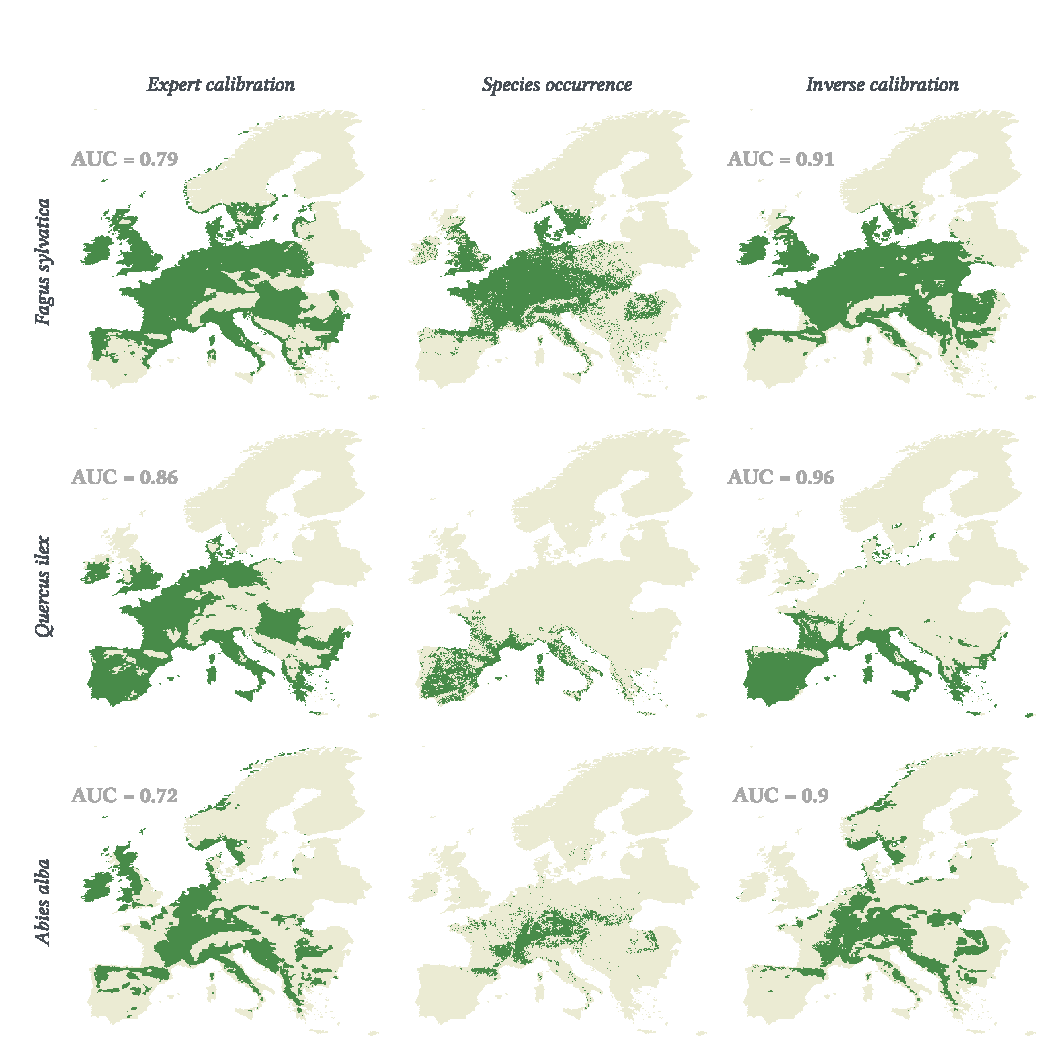
\includegraphics{chapter1/figs/phenofitmaps} 
\caption{\textbf{Species distribution maps obtained with PHENOFIT expert and inverse calibrations, compared with observed species occurrences.} Optimal threshold to dichotomize model predicted fitness index in presence/absence is the Youden index-based cut-off point. Note that models predict species climatic niche which is larger than the realized niche that corresponds to species presence map.}
\label{fig:phenofitmaps}
\end{figure}

\begin{figure}
\centering 
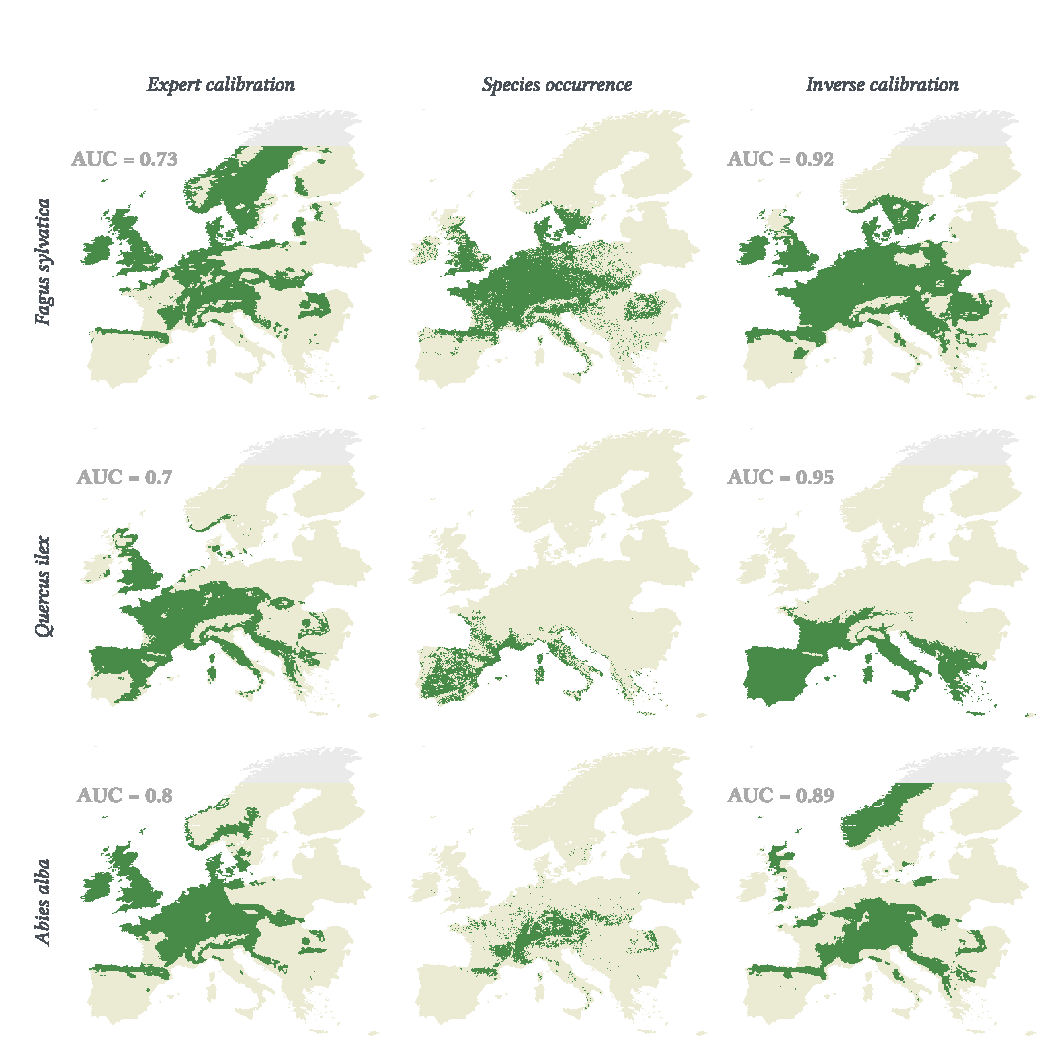
\includegraphics{chapter1/figs/castaneamaps} 
\caption{\textbf{Species distribution maps obtained with CASTANEA expert and inverse calibrations, compared with observed species occurrences.} Optimal threshold to dichotomize model predicted carbon reserves in presence/absence is the Youden index-based cut-off point. Note that models predict species climatic niche which is larger than the realized niche that corresponds to species presence map. Note also that CASTANEA cannot be used in high-latitude regions (grey area).}
\label{fig:castaneamaps}
\end{figure}

\subsubsection{Impacts of subsampling and calibration
stochasticity}\label{impacts-of-subsampling-and-calibration-stochasticity}

\paragraph{Variability of calibration
performance}\label{variability-of-calibration-performance}

The 100 calibrations of the PHENOFIT model realized for beech showed
that random data subsampling had an effect on the final objective
function value (i.e.~the AUC computed on the 2000 calibration points).
Kruskal-Wallis test was significant (p = 2.1e-08), meaning that at least
one subset provided better AUC during calibration. According to Dunn's
tests, 11 pairwise comparisons out of 45 were significant
(\Cref{fig:cmaesrepAUCcal}). The calibration AUC ranged
from 0.879 to 0.923 over all subsets, with a mean value of 0.9.

However, more importantly, the repetition of calibrations on different
subsets had no significant impact on the total AUC computed on all
presence/absence points (Kruskal-Wallis test, p = 0.96). Thus, no subset
led to an overall better prediction of the species distribution (see
\Cref{fig:cmaesrepAUCcal}). The total AUC ranged from
0.881 to 0.914, with a mean value of 0.896. \newline

\begin{figure}[H]
\centering 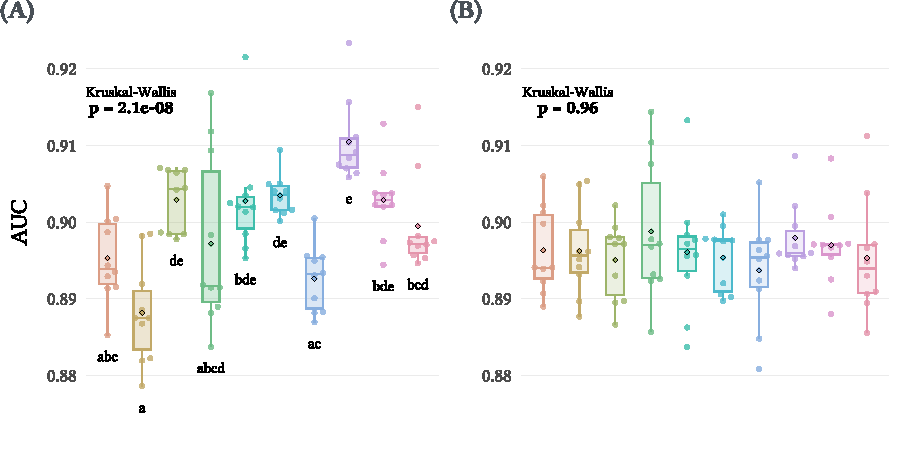
\includegraphics{chapter1/figs/cmaesrepAUCcal} 
\caption{\textbf{Effects of data sub-sampling and stochasticity on CMA-ES calibration using the PHENOFIT model for beech.} \textbf{(A)} calibration AUC (calculated only with calibration cells) and \textbf{(B)} total AUC (calculated with all presence/absence cells). Each color is a different sub-sampling of occurrence data, each point is a calibration run. Diamonds (with black border) are mean AUC values. On \textbf{(A)}, the grouping letters represent the multiple comparisons with pairwise Dunn’s tests.}\label{fig:cmaesrepAUCcal}
\end{figure}

\paragraph{Non-identifiability of
parameters}\label{non-identifiability-of-parameters}

To illustrate the variability in the parameter estimates that can be
obtained with the inverse calibration, we focused on the leaf unfolding
date submodel of PHENOFIT (see \hyperref[chap1:appendixA]{Appendix A}
and \hyperref[chap1:appendixG]{Appendix G}). The parameter values
found by CMA-ES varied greatly across the 100 calibrations
(\Cref{fig:unfoldingplots}). For example, the critical
amount of chilling \(C_{crit}\) required to break bud dormancy and the
critical amount of forcing \(F_{crit}\) required to break bud ranged
from 1.02 to 149.96 and from 1.5 to 79.26 respectively, with a mean
value of 51.52 and 38.78. Their coefficient of variations were 126.7\%
and 51.9\% respectively. Kendall correlation coefficient between
\(C_{crit}\) and the threshold temperature of the response function to
temperature during dormancy \(T_b\) is 0.64 (\(p <\) 0.001). Kendall
correlation coefficient between \(F_{crit}\) and the mid-response
temperature \(T_{50}\) is -0.55 (\(p <\) 0.001).

\clearpage

\begin{figure}[H]
\centering 
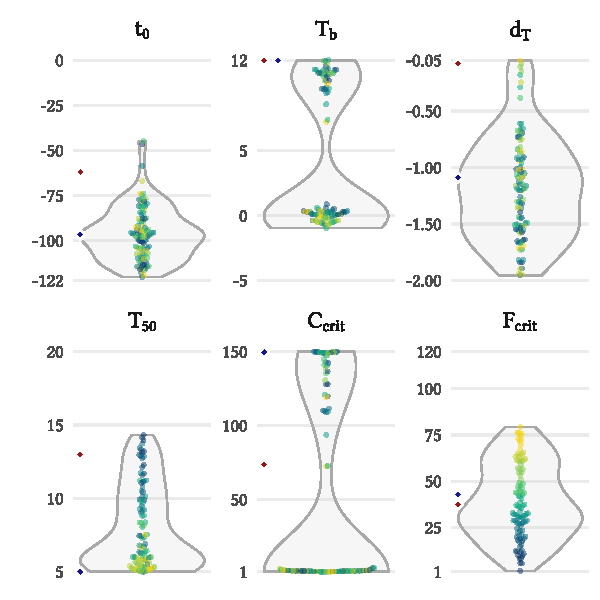
\includegraphics{chapter1/figs/unfoldingplots} 
\caption{\textbf{Effects of stochasticity of CMA-ES calibration on PHENOFIT leaf unfolding model parameter values for beech.} Each panel is a parameter. Y-axis limits are lower and upper bounds used during calibration. Each point is a calibrated parameter value, color gradient is based on $F_{crit}$ values. Red diamonds are parameter values obtained with expert calibration, blue ones are parameter values obtained with the best inverse calibration.}\label{fig:unfoldingplots}
\end{figure}

\subsection{Discussion}\label{discussion}

Our results showed that CMA-ES is an efficient optimizer for inverse
calibration of complex ecological models. The algorithm was able to find
parameter sets that significantly improved the predictions of the
calibrated models compared to the expert parametrization. However, our
study also highlighted the issue of non-identifiability of parameter
values due to the data limitation and the dependence between
process-explicit model parameters, which may result in diverging parameter
values even though the calibrated models describe the observed species
distribution well.

\subsubsection{Performance and advantages of CMA-ES to calibrate
complex models}\label{performance-and-advantages-of-cma-es-to-calibrate-complex-models-in-ecology}

Here we demonstrated that inverse calibration with CMA-ES is feasible
and provide good results for complex and runtime-expensive ecological
models.\\
With a subsampling of species occurrence data, the algorithm succeeds in
finding parameter sets which provide higher AUC values. The predictions
of the calibrated models are sharply improved compared to expert
parametrization (\Cref{fig:phenofitmaps,,fig:castaneamaps}). Two striking examples are the
increase in the performance of PHENOFIT model for silver fir, from 0.72
to 0.9, and of CASTANEA model for holm oak, from 0.7 to 0.95. Moreover,
CMA-ES performed equally well regardless of the species occurrence
subset used during calibration
(\Cref{fig:cmaesrepAUCcal}), and thus permitted to find
a good compromise between computational cost and calibration efficiency.

CMA-ES is a ``generic'' optimizer which can be applied to various
problems. It is easy to use as it does not require an extensive tuning
to efficiently explore the parameter space. We only had to choose the
number of candidate solutions \(\lambda\), and the initial search region
(initial starting point and step size \(\sigma\)). As well as being
quasi parameter-free, CMA-ES has several structural advantages
particularly useful for complex optimization problems. First, the
algorithm's covariance matrix enables the learning of second-order
information, which provides insights into pairwise dependencies between
parameters. Second, the covariance matrix adaptation of CMA-ES is highly
efficient in handling ill-conditioned and non-separable problems
\citep{Hansen2011}. Last,
CMA-ES's update mechanism of step size \(\sigma\) (i.e.~the mutation
force) helps prevent premature convergence
\citep{Hansen2001},
allowing the algorithm to explore more of the search space. CMA-ES has
been shown to outperform several other optimization algorithms
\citep{Hansen2010}, and is
usually the most efficient method when the target cost (i.e.~the number
of objective function evaluations) is about \(100*N\) (\(N\) being the
dimension of the parameter search space,
\citealp{Baeck2013}).

\subsubsection{Non-identifiability of parameter values}\label{non-identifiability-of-parameter-values}

Equifinality is a common problem encountered during model calibration,
where multiple parameter sets can produce equally good fits to the
observed data. This issue can arise due to several factors, including
limitations in the quantity or quality of available data, competing
processes within the model, and parameter interactions that affect the
model output in complex ways.

In both models used in this study, biological mechanisms are explicitly
calculated in several submodels (e.g.~a leaf unfolding submodel or a
stomatal opening submodel). A submodel output has inevitably a
significant influence on the other submodels as biological processes can
be highly dependent with feedbacks: in CASTANEA, for example, the
stomatal opening affects the photosynthesis, and \emph{vice versa}.
Within each submodel, parameters are also strongly dependent because of
structural correlations. To illustrate this problem, we focused on the
beech leaf unfolding submodel of PHENOFIT (see
\hyperref[chap1:appendixA]{Appendix A}). This model has 6 parameters
\citep{Chuine2000}: a starting date of
the processes (\(t_0\)), one parameter describing the response function
to temperature during the dormancy phase (\(T_b\)), two parameters
describing the response function to temperature during the phase of bud
growth (\(d_T\), \(T_{50}\)), and two parameters representing the sums
of the daily responses to temperature during bud dormancy (\(C_{crit}\))
and during bud growth (\(F_{crit}\)) that respectively determine the
date of bud dormancy break and the date of leaf unfolding (see
\hyperref[chap1:appendixG]{Appendix G} for details). Since no
information on the date of bud dormancy break is available for the
calibration, a first structural negative correlation exists between
\(C_{crit}\) and \(F_{crit}\): the same leaf unfolding date can be
obtained with either a long dormancy phase and short bud growth phase or
a short dormancy phase and a long bud growth phase. Other structural
correlations exist between \(T_b\) and \(C_{crit}\) on the one hand and
\(d_T\)/\(T_{50}\) and \(F_{crit}\) on the other hand: for example, a
rapid accumulation of chilling units with a high critical chilling
requirement could yield identical results as a slow accumulation with a
low critical chilling requirement (i.e.~the threshold temperature
\(T_{b}\) and the critical chilling requirement \(C_{crit}\) are
dependent, see \hyperref[chap1:appendixG]{Appendix G}).

Consequently, several parameter sets may be statistically equivalent and
parameters non-identifiable. In fact, calibration repetitions gave
diverging parameter values (\Cref{fig:unfoldingplots})
while being efficient in distinguishing between species presence and
absence (i.e.~AUC \textasciitilde{} 0.9,
\Cref{fig:cmaesrepAUCcal}). Thus, even if the calibrated
model describes the observed species distribution very well, it does not
necessarily mean that parameter values are ecologically relevant. This
concern is similar to the criticisms against correlative SDMs, in which
parameter values and correlations that well reproduce species ranges do
not necessarily describe a complex biological reality. In our case, the
constraints imposed by the explicit mathematical equations embedded in
the models we used were not sufficient to ensure calibration convergence
towards similar solutions that would have suggested a high biological
realism. However, it is worth noting that we deliberately chose large
parameter ranges (although biologically realistic, i.e.~corresponding to
the observations made on the different processes modelled across
different species) in order to give free rein to the optimization
algorithm. As our goal was to assess the performance of CMA-ES
objectively, we did not attempt to minimize this non-identifiability
issue by restricting the parameter space. To deal with equifinality
issues, an avenue to explore could be the use of multiple objective
functions during model calibration to assess different aspects of the
model performance. Additionally, if a closed-form likelihood can be
derived, one could use a Bayesian framework to combine prior knowledge
and inverse estimation of parameters to constrain the parameter space
and study the nature of trade-offs between parameters
\citep{Hartig2012, Cailleret2020}.

\subsubsection{Methodological issues and perspectives}\label{methodological-issues-and-perspectives}

Our goal here was to investigate the performance of CMA-ES to calibrate
quite complex process-explicit species distribution models using species
occurrence data. We did not attempt to validate our parametrizations
using temporally or spatially independent data, and AUC was only used to
determine if model outputs were consistent with species distributions.
However, AUC is scale-invariant: it measures how well predictions are
ranked rather than their absolute values. For example, with PHENOFIT, a
species with a fitness of \(0.8\) could be considered as absent while
another one with the same fitness could be considered as present.
Therefore, when it is used as an objective function for model
calibration, we probably lack some precision and consistency among
species' parameters estimation. Further work could thus be conducted to
examine the effects of choosing a different objective function.

It would also be valuable to use a significantly higher computing power,
with an adapted version of CMA-ES. To improve the global search
performance of CMA-ES, we slightly increased the number of candidate
solutions \(\lambda\) \citep{Hansen2004} and used a computing cluster to evaluate \(\lambda\) functions in
parallel. We were able to use between 40 and 120 cores, which is far
from the computing power of some GPUs (\textgreater{} 2000 cores). In
this case, choosing a very large number of candidate solutions might not
be the best choice. To use efficiently this large parallel computing
power, one could rather use a CMA-ES restart strategy \citep[e.g. IPOP-CMA-ES,][]{Auger2005}, where the
number of candidate solutions is successively increased (by a factor of
2), and run these calibrations in parallel. Moreover, when a model
requires a high computation time and thus only a small budget can be
afforded, the original fitness function could be approximated with a
surrogate model in order to reduce the number of original function
evaluations required \citep[e.g.][]{Auger2004, Loshchilov2013}. 

There are several issues regarding the process-explicit models we used
which can impact their calibration and bias their parameter estimates.
First, like any model, although they have a certain level of complexity,
they are not a perfect representation of the reality, and their inherent
structural errors increase the probability of finding parameter values
that deviate from the true values of the underlying processes \citep[see][]{Oberpriller2021}. Second, they do not necessarily include all the environmental
factors at stake. For example, pedologic variable in PHENOFIT only
involve the water holding capacity. In this model, other variables such
as pH or soil texture are not considered. Third, and more importantly,
they are used here to represent the fundamental niche, and to estimate
the potential distribution of the species using pedoclimatic variables.
When calibrated against observed distributions, which represent the
realized niche, they face the same issues as correlative models, and
their parameter estimated can be distorted because compensating for
processes not represented in the model (e.g. biotic interactions). In
addition, in our case here, land use management probably also play an
important role in shaping tree realized distribution, while not being
addressed in the models. We included GBIF occurrence data, and
especially as much as possible isolated native tree records outside
forests, to help correct this problem, but it is impossible to be
exhaustive at the spatial resolution of 0.1°. At this scale, local
variations of soil characteristics and of competitive interactions among
trees (e.g.~along an altitudinal gradient) can also not be considered.

Finally, several authors advocate for process-explicit modeling approaches
relying upon species response functions that are a priori defined \citep[e.g.][]{Higgins2020}.
However, the main limitation of such models is the data availability to
infer their parameters \citep{Urban2016}. Expert parameterization is often long and arduous. One
possible way to facilitate parameter value estimation would be to use
inverse calibration, and we demonstrated here that CMA-ES can be a
powerful optimizer to this end. For example, CMA-ES driven by species
occurrence data could be used to calibrate submodels whose parameter
values cannot be measured or are too hard to measure experimentally.
However, when a structural correlation exists (i.e.~trade-off between
processes that are inherently present and interconnected in the model,
as in the leaf unfolding submodel), inverse calibration might not
provide the right parameter estimates. In such a case, expert knowledge,
observations and measurements are necessary to determine \emph{a
posteriori} which estimates are the most realistic. This is possible in
the case of process-explicit SDMs, and usually not feasible in the case of
correlative SDMs. A combination of both expert and inverse calibrations
might offer a new perspective for spreading the use of process-explicit
models in predictive ecology, especially for climate change impact
studies.

\clearpage

\subsection{Acknowledgements}\label{acknowledgements}

The authors would like to thank Hendrik Davi for helping us in using the
CASTANEA model. We are also deeply grateful for many helpful comments
from Florence Tauc. We would also like to thank François de Coligny,
manager of the CAPSIS platform, Gilles Le Moguedec, and the GenOuest and
TGCC teams for their support. Finally, we would like to thank Florian
Hartig and another anonymous reviewer whose comments and suggestions
helped us improve and clarify this manuscript.\\
V.V. was supported by a GAIA doctoral school PhD Fellowship.

\subsection{Author contributions}\label{author-contributions}

I.C. devised the main conceptual ideas. V.V. worked out the technical
details, performed the numerical calculations and wrote the first draft
of the manuscript. The two authors discussed the analyses and the
results, and contributed to the final manuscript.

\subsection{Data availability}\label{data-availability}

ERA5-Land dataset is available on the
\href{https://cds.climate.copernicus.eu/cdsapp\#!/dataset/reanalysis-era5-land?tab=overview}{Copernicus
Climate Change Service website}. EU-SoilHydroGrids is available on the
\href{https://esdac.jrc.ec.europa.eu/content/3d-soil-hydraulic-database-europe-1-km-and-250-m-resolution}{European
Soil Data Centre website}. SoilGrids250m is available on the
\href{https://www.isric.org/explore/soilgrids}{International Soil
Reference and Information Centre website}. EU-Forest database is
available on
\href{https://figshare.com/collections/A_high-resolution_pan-European_tree_occurrence_dataset/3288407}{FigShare}.
The R code associated with this work is available on
\href{https://github.com/vvandermeersch/inverse_calibration}{this GitHub
repository}, as well as on Zenodo
(\href{https://doi.org/10.5281/zenodo.7774981}{10.5281/zenodo.7774981}).